\section{Results}
\label{sec:results}

\begin{table*}[ht]
    \centering
    \caption{Creation time, new file size, and index size using the sync point
    strategy.}
\begin{tabular}{l|r|r|r}
   
    File & Creation Time (s) & New File Size (B) & Index Size (B)\\
    \hline
    Small & 187 & 198,095,562 &  4608\\
    Medium & 1164 & 2,204,279,194 &  67032\\
    Large & 1441 &  3,546,205,784 &127848\\
    XL & 2137 & 5,341,584,427 & 171624\\
\end{tabular}
    \label{tab:sync}
\end{table*}


In this section we discuss the results of using our \ibuilder to create index
files over variously-sized \gzip FASTQ files, and then turn to the results of
running \ireader on those index files. We also give results of the construction
time of our sync point index.

\subsection{Building Indices}
\label{sec:buildresults}

\begin{figure*}%
\centering
    \begin{subfigure}[c]{.48\textwidth}
        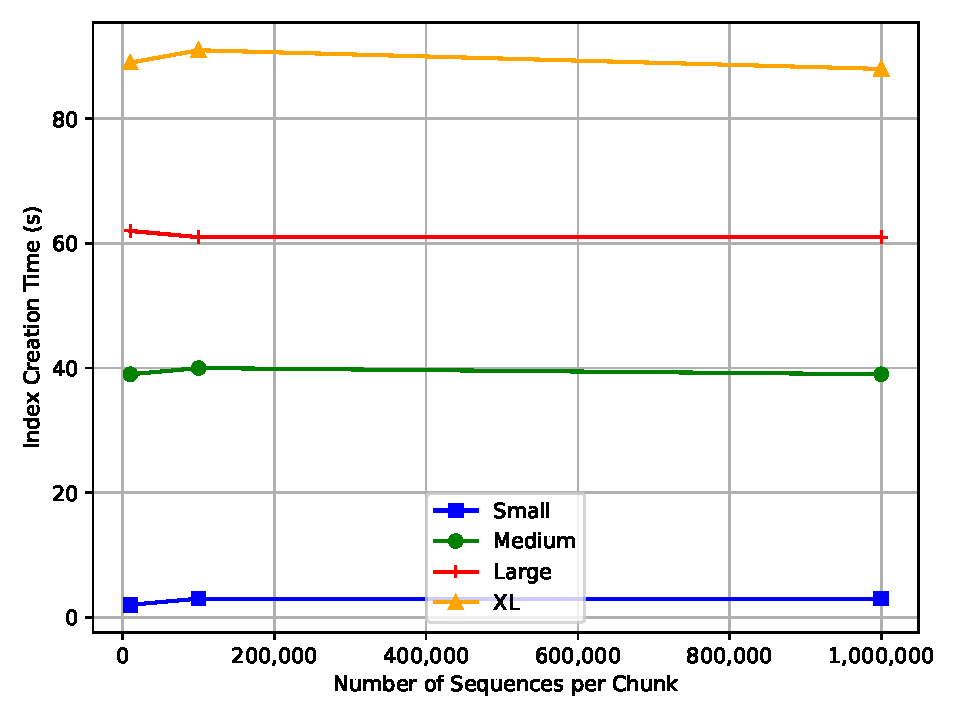
\includegraphics[width=\linewidth]{figs/creation-time.pdf}
        \caption{The number of seconds required to construct the index.}
        \label{fig:creation}
    \end{subfigure}%
    \begin{subfigure}[c]{.48\textwidth}
        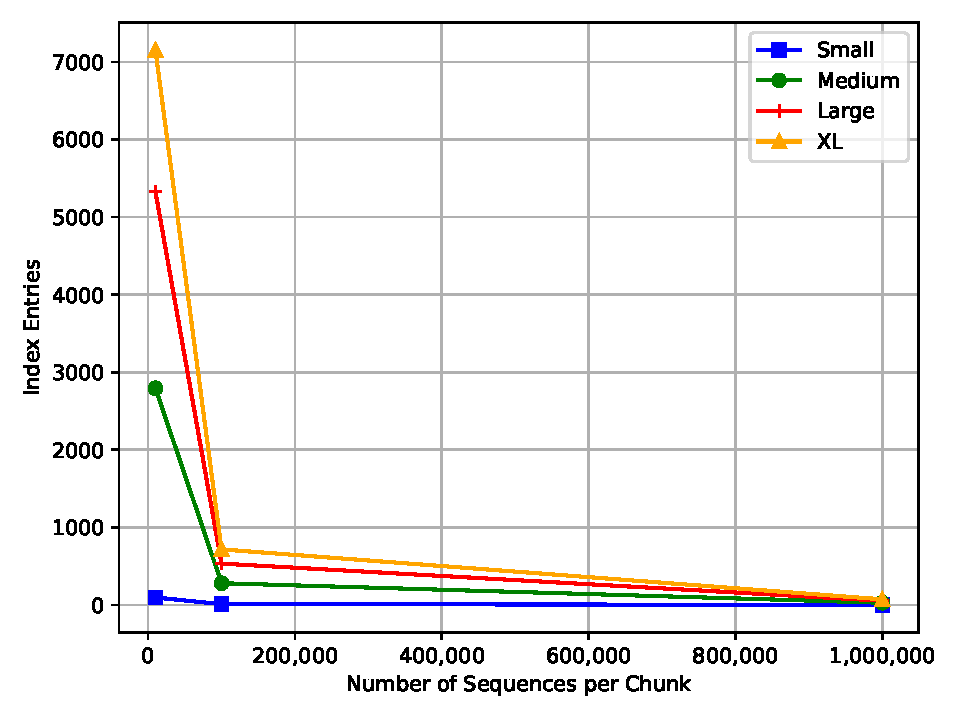
\includegraphics[width=\linewidth]{figs/index-entries.pdf}
        \caption{The number of entries in the index.}
        \label{fig:entries}
    \end{subfigure}%
    \hfill
    \begin{subfigure}[c]{.48\textwidth}
        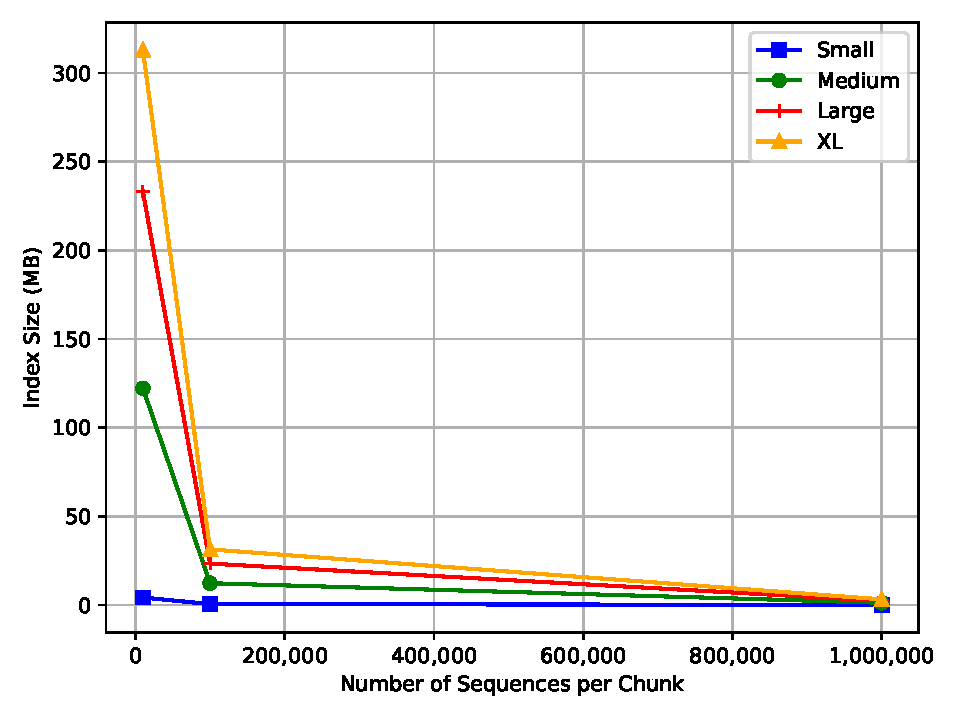
\includegraphics[width=\linewidth]{figs/index-bytes.pdf}
        \caption{The number of bytes in the index.}
        \label{fig:bytes}
    \end{subfigure}%
    \begin{subfigure}[c]{.48\textwidth}
        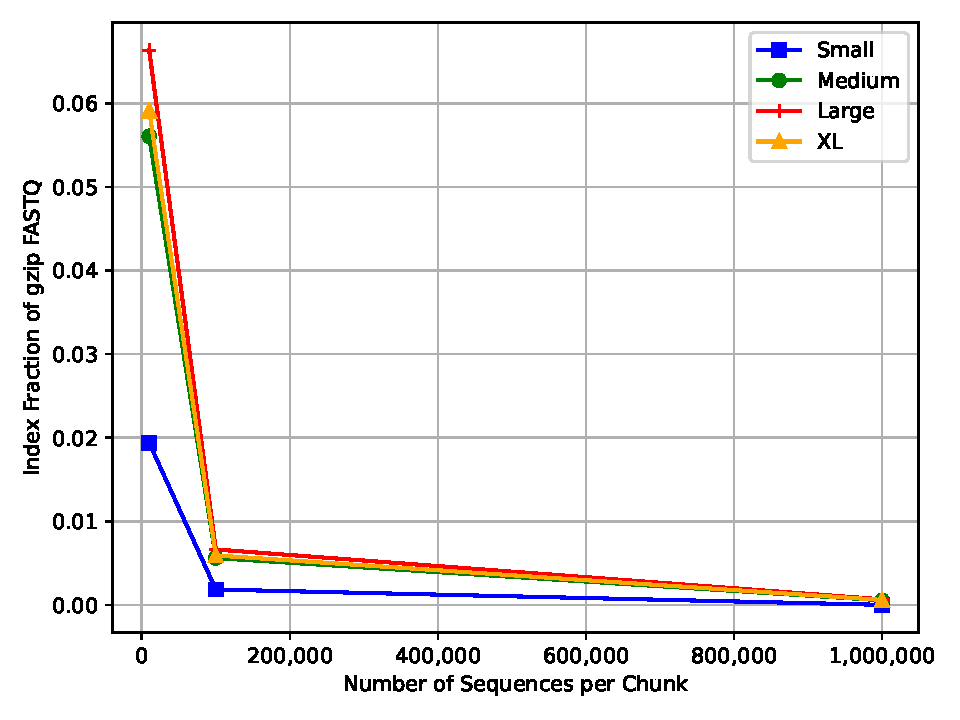
\includegraphics[width=\linewidth]{figs/index-frac.pdf}
        \caption{The index size divided by the \gzip FASTQ file size.}
        \label{fig:frac}
    \end{subfigure}%
    \caption{Metrics for our \gzip FASTQ index builder; S, M, L, and XL refer to
    the four \gzip files and their relative sizes. See Table~\ref{tab:source}.}
    \label{fig:builder}
\end{figure*}

Using the \gzip FASTQ samples we described in Table~\ref{tab:source}, we run
\ibuilder over each. For each sample, we record the time it takes to build the
index files, the number of indices that each file contains, and the number of
bytes in each of the resulting indexes. Figure~\ref{fig:builder}'s subplots
contain graphical representations of these measurements. All measurements were
conducted on a 16 core Dell Precision 5560 with an 11th Gen Intel Core i7-11850H
\@ 2.50GHz running Kubuntu 22.04 LTS.

Figure~\ref{fig:creation} displays the creation times associated with each file
size while varying the number of sequences in each chunk between 10,000,
100,000, and 1,000,000. Index creation time increases roughly linearly as the
\gzip FASTQ file the index is being built over increases. This matches our
intuition because \ibuilder simply reads the \gzip file from start to finish,
decompressing the data in 32kB chunks as it goes. Larger files require longer to
read. Keeping the file size fixed, the times to write the index files do not
drastically change as we increase the number of sequences per chunk. This is
because the vast majority of our index building time is spent reading the file
and creating the index points. Because we always have to scan the inflated
buffer for newlines to count sequences, and because creating an index point is a
relatively low-cost operation, creating less index points does not save much
time in the overall \ibuilder runtime.

Figure~\ref{fig:entries} depicts the number of index points generated by
creating indexes over our data sources using different sequence chunk counts. In
all of our experiments there was a one-to-one correspondence between the number
of \gzip DEFLATE block index points and sequence chunk index points -- that is,
there were never instances in which two different sequence chunks started within
the same DEFLATE block. This could happen if the sequence number chunk size
specified was relatively small; we considered this a pathological case as we
believed the number of parallel readers would be relatively small (O(10)). This
argues for larger sequence number chunks, rather than smaller. The numbers
reported here thus represent both the number of DEFLATE block index points as
well as the number of sequence chunk index points. Unsurprisingly, as the number
of sequences per chunk increases, the number of index points we create decreases
drastically.

Figure~\ref{fig:bytes} shows how the size of the index files changes as the
sequence chunk number changes. Both the \texttt{.idx} and \texttt{.seq-idx} are
combined for each file size/sequence chunk size data point. Because each index
point requires storing a 32kB buffer in order to initialize the \zlib
decompression from an index point, when more index points are built the index
files grow large. At a sequence chunk size of 10,000, the size of the index
files for all \gzip FASTQ references are more than 100MB except for the
smallest. As the number of index points created decreases as the number of
sequences per chunk increases, however, the size of all of the index files grows
quite small. The 1,000,000 sequence chunk index size for the XL FASTQ reference
is only 3 MB, which is smaller than the 4 MB S index size at the 10,000 reads
per chunk level. This suggests if optimizing disk space is a priority, larger
sequence chunks should be used.

Figure~\ref{fig:frac} plots the index size relative to the original \gzip file.
The shape of this plot follows the preceding subfigures. As the number of
sequence reads per index point increases from 10,000 to 1,000,000, the size of
the index file relative to the original \gzip drops from more than 5\% in the
case of the M, L, and XL source files, to around 0.05\%.

\subsection{Parallel Reading}
\label{sec:readresults}

\begin{figure}[h]
    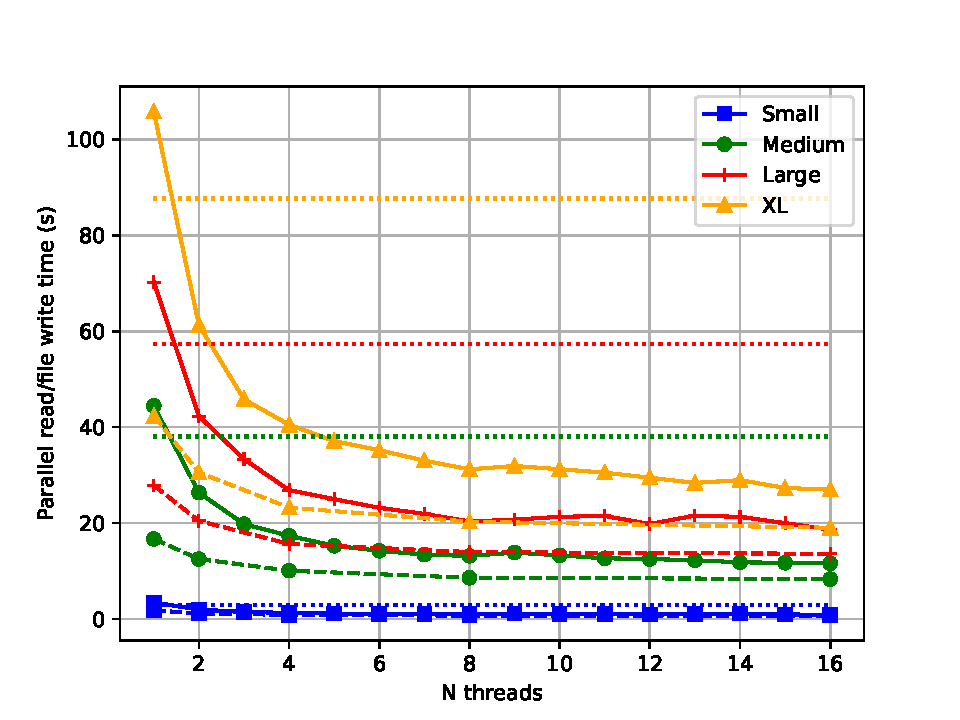
\includegraphics[width=\linewidth]{figs/threads.pdf}
    \caption{Time to read differently-sized FASTQ \gzip files using a pre-built
    index file and different numbers of threads. Time compasses total program
    execution, including reading the index files, parallel reading the \gzip
    file with $N$ threads, and writing the reconstituted file to disk. Time for
    \texttt{zcat} to read the file and write it to disk is shown for comparison
    using a dotted line (\texttt{zcat} execution is single threaded). Another
    parallel (but not ``sequence aware'') gzip reader implementation
    \texttt{pugz} is shown in a dashed line. See
    Table~\ref{tab:source} for descriptions of small, medium, large, and XL.}
    \label{fig:threads}
\end{figure}

Using the index files we generated for each of the data sources we considered,
we read each of the files in parallel using a variable number of threads. We
used POSIX threading library \texttt{libpthread} to implement our parallel,
multithreaded reading approach.

For each file, we used \ireader and varied the thread parameter \texttt{-n
N\_THREADS} between 1 and 16 to test the runtime of the parallel reader. After
each iteration, we used GNU \texttt{diff} to ensure that the resulting file
produced by our parallel reader was the same as the original, uncompressed FASTQ
file (that is, that \ireader introduced no errors.) In all instances, our
parallel reader produced the correct, uncompressed output file.

We compared our \ireader implementation's execution time with a varying number
of threads against \texttt{zcat}. \texttt{zcat} is another \zlib utility that
decompresses a \gzip file and writes the result to standard out. Importantly,
\texttt{zcat} is a single-threaded application. In our data, we compare the
amount of time it takes \texttt{zcat} to inflate a file, which we write to
standard out to provide the best comparison against our \ireader utility.

Figure~\ref{fig:threads} displays the total \ireader runtime using a varying
number of threads for each file size using solid lines. The dotted lines
represent the amount of time it took to use the \texttt{zcat} tool to read the
file in serial and redirect its output to a file. The dashed lines represent
parallel \gzip reading using a non-sequence aware implementation called
\texttt{pugz}.

Our \ireader implementation using only a single thread (non-parallel) underperformed
\texttt{zcat} at each file size by approximately 10-20\% for the three larger
file sizes. This is likely due to our implementation continuing to count lines
and sequences within the \gzip file it is inflating, despite there being no need
to do so with only a single thread -- it is reading the entire file. When the
number of threads increases so that there are parallel readers ($>$1 threads),
we outperform our \texttt{zcat} baseline at every file size and number of
threads. At only two threads, our parallel reader takes 69\% of the
\texttt{zcat} time (61.2 seconds vs 87.65 seconds) for the XL data source, and
only 30\% of the \texttt{zcat} time at 16 threads. A clear knee between $2 \leq
N \leq 4$ threads is observed; adding more than four threads exhibits clear
diminishing returns.

\subsection{Sync Point Index}

We also evaluated the performance of our sync point index for the same four data 
sources across multiple construction-time metrics, namely the time taken to simultaneously 
recompress the file and build the index, the size of the recompressed file, and the size of 
the index. The results are shown in Table~\ref{tab:sync}. As expected, we found that index 
creation time is far longer than that of our \ibuilder tool because we need to read, decompress, 
recompress, and write the entire file. In terms of the \gzip size after recompression, we found 
that sync point insertion increases the file size by approximately 5-6\%, regardless of the 
original \gzip size. While the percentage increase is relatively small, for large \gzip files, 
the amount of extra bytes can still exceed the space savings provided by the minuscule index 
sizes. Even for the largest file tested, the resulting index size is less than 200 KB.

Unfortunately, our parallel reader implementation for the sync point index is significantly less 
efficient than all other implementations tested, taking minutes to parse even the medium file with 
16 threads. We uncertain as to the exact cause of the inefficiency; however, we note that the primary 
questions regarding the feasibility of the sync point index were based on its construction as opposed 
to using it to read chunks in parallel. With a more optimal parallel reader implementation, we may 
see that the execution time to read \gzip files in parallel competes with those of our \ibuilder tool
and other existing decompression tools.
